\documentclass[openany, twoside, a4paper, 12pt]{extbook}

\usepackage[utf8]{inputenc}
\usepackage{rotating}
\usepackage[russian]{babel}
\usepackage{amsfonts} 
\usepackage{amstext}
\usepackage{amssymb}
\usepackage{amsthm}
\usepackage{graphicx} 
\usepackage{subfig}
\usepackage{color}
\usepackage{svg}
\usepackage{epstopdf}
\usepackage[unicode]{hyperref}
\usepackage[nottoc]{tocbibind} 
\usepackage{verbatim}
\usepackage{listings}
\usepackage{indentfirst}
\usepackage{commath}
\usepackage[colorinlistoftodos, prependcaption]{todonotes}
\usepackage{multirow}
\usepackage{algorithmic}
\usepackage{algorithm}
\usepackage{amsmath}

\title{Задача оптимизации расписания с использованием алгоритма имитации отжига}
\author{Санников Тимофей Владимирович}

\begin{document}

	\maketitle
	\section*{Формальная постановка}
	\subsection*{Дано:}
	
	\begin{itemize}
	    \item \( N \) — количество независимых работ.
	    \item \( M \) — количество процессоров.
	    \item \( t_i \), \( i = 1, 2, \dots, N \) — время выполнения каждой работы \( i \), \( t_i > 0 \).
	\end{itemize}
	
	\subsection*{Требуется:}
	
	Построить расписание выполнения всех
	\( N \) работ на \( M \) процессорах без прерываний,
	чтобы минимизировать критерий указанный далее~\ref{cr1}.


	\subsection*{Расписание}

	Расписание представлено в виде булевой матрицы размера $ M \mod N $,
	в которой стоит 0 в случае если работа не выполняется на процессоре,
	1 если выполняется.

	Для каждого процессора при помощи матрицы определяется $ \mathcal{J}_j $,
	обозначающее множество всех работ определенных на выполнение на данном процессоре.
	Тогда $ T_j = \sum_{i \in \mathcal{J}_j} t_i $ --- время выполнения всех назначенных на процессор \( j \) работ.
	Причем, учитывая что все работы будут выполнены, $ \sum_{j=1}^{M} \mathcal{J}_j = N$

	Приведем пример расписания~\ref{rasp}. 
	В данном примере:
	\begin{itemize}
		\item 1-ая задача выполняется 2 процессором, 
		\item 2-ая задача выполняется 1 процессором,
		\item 3-ая задача выполняется 3 процессором,
		\item 4-ая задача выполняется M процессором,
		\item N-1-ая задача выполняется M процессором,
		\item N-ая задача выполняется другим процессором.
	\end{itemize}
	\begin{table}
			\begin{tabular}{|p{1.8cm}|p{1.8cm}|p{1.8cm}|p{1.8cm}|p{1.8cm}|p{1.8cm}|} 
		\hline
		& 1 & 2 & 3 & \ldots & $ M $ \\ 
		\hline
			1 & 0 & 1 & 0 & \ldots & 0 \\ 
		\hline
			2 & 1 & 0 & 0 & \ldots & 0 \\ 
		\hline
			3 & 0 & 0 & 1 & \ldots & 0 \\ 
		\hline
			4 & 0 & 0 & 0 & \ldots & 1 \\ 
		\hline
			\ldots & \ldots  & \ldots  & \ldots  & \ldots & \ldots  \\ 	
		\hline
			$N-1$ & 0 & 0 & 0 & \ldots & 1 \\ 
		\hline
			$N$ & 0 & 0 & 0 & \ldots & 0\\ 
		\hline
	\end{tabular}
		\caption{Пример расписания}
		\label{rasp}
	\end{table}

	\subsection*{Минимизируемый критерий:}
		
	Критерий выбирается на основе значения контрольной суммы CRC32 от фамилии и инициалов:
	\begin{itemize}
		\label{cr1}
	    \item Остаток от деления CRC32 на 2 равен 1: минимизируется \( K_1 \).
	    \item Остаток от деления CRC32 на 2 равен 0: минимизируется \( K_2 \).
	\end{itemize}
	CRC32 для моего имени и инициалов = 2613818349, что означает, что мой критерий --- К1
	

	Критерий \( K_1 \): Разбалансированность расписания
	\[
	K_1 = T_{\text{max}} - T_{\text{min}},
	\]
	где:
	\[
	T_{\text{max}} = \max_{j=1, 2, \dots, M} T_j,
	\]
	\[
	T_{\text{min}} = \min_{j=1, 2, \dots, M} T_j,
	\]

	\subsection*{Дополнительные условия:}
	
	Расписание должно удовлетворять следующим ограничениям:
	\begin{itemize}
	    \item Каждая работа выполняется на одном процессоре без прерываний.
	    \item Одна работа не может быть запущена на нескольких процессорах одновременно.
	    \item Время выполнения каждой работы \( t_i \) фиксировано.
	\end{itemize}
	\section*{Исследование последовательного алгоритма}
	Для Исследования работы последовательного алгоритма
	был проведен запуск программы, получающей на вход 
	различное количество задач, число которых росло пока время распределения по процессорам
	не достигло одной минуты.
	Задачи имели случайно сгенерированное время выполнения от 1 до 100.
	Полученные наборы задач были распределены с использованием различных законов понижения температуры.

	\begin{figure}[h]
	    \centering
	    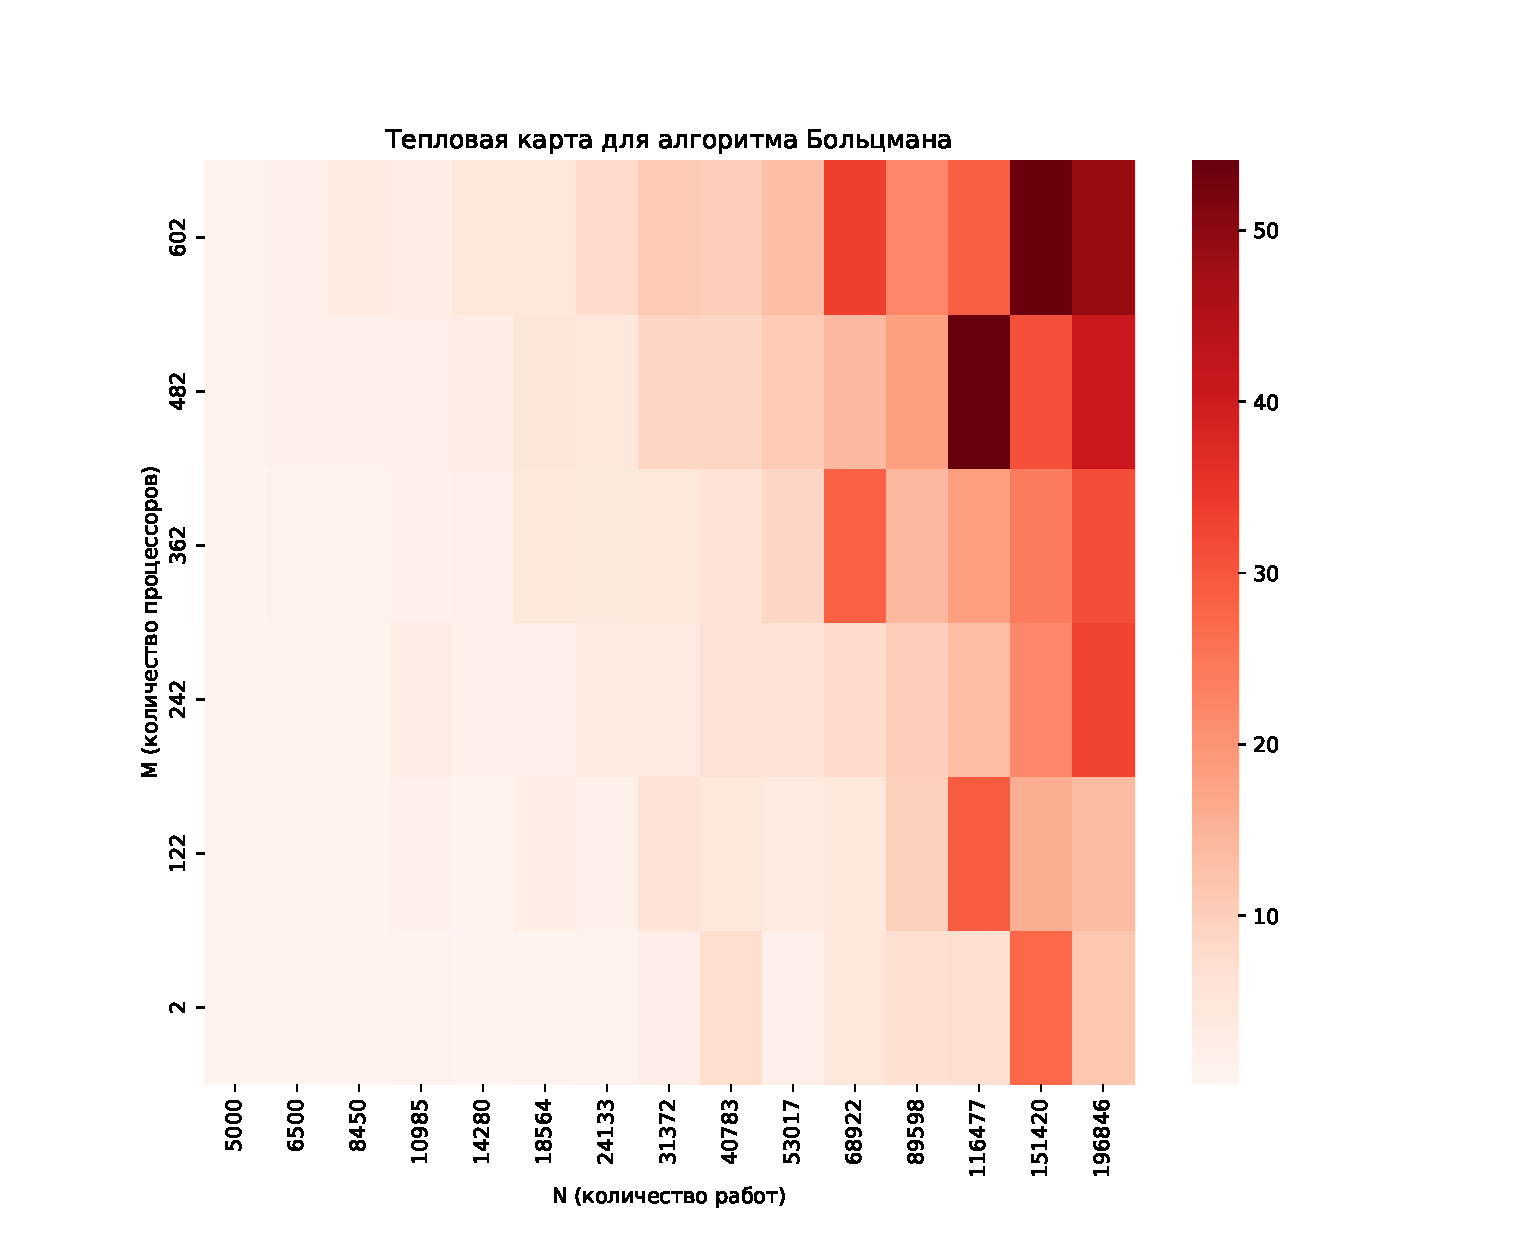
\includegraphics[width=\textwidth]{boltzmann_heatmap.eps}
	    %\caption{}
	    \label{fig:boltzmann}
	\end{figure}
	
	\begin{figure}[h]
	    \centering
	    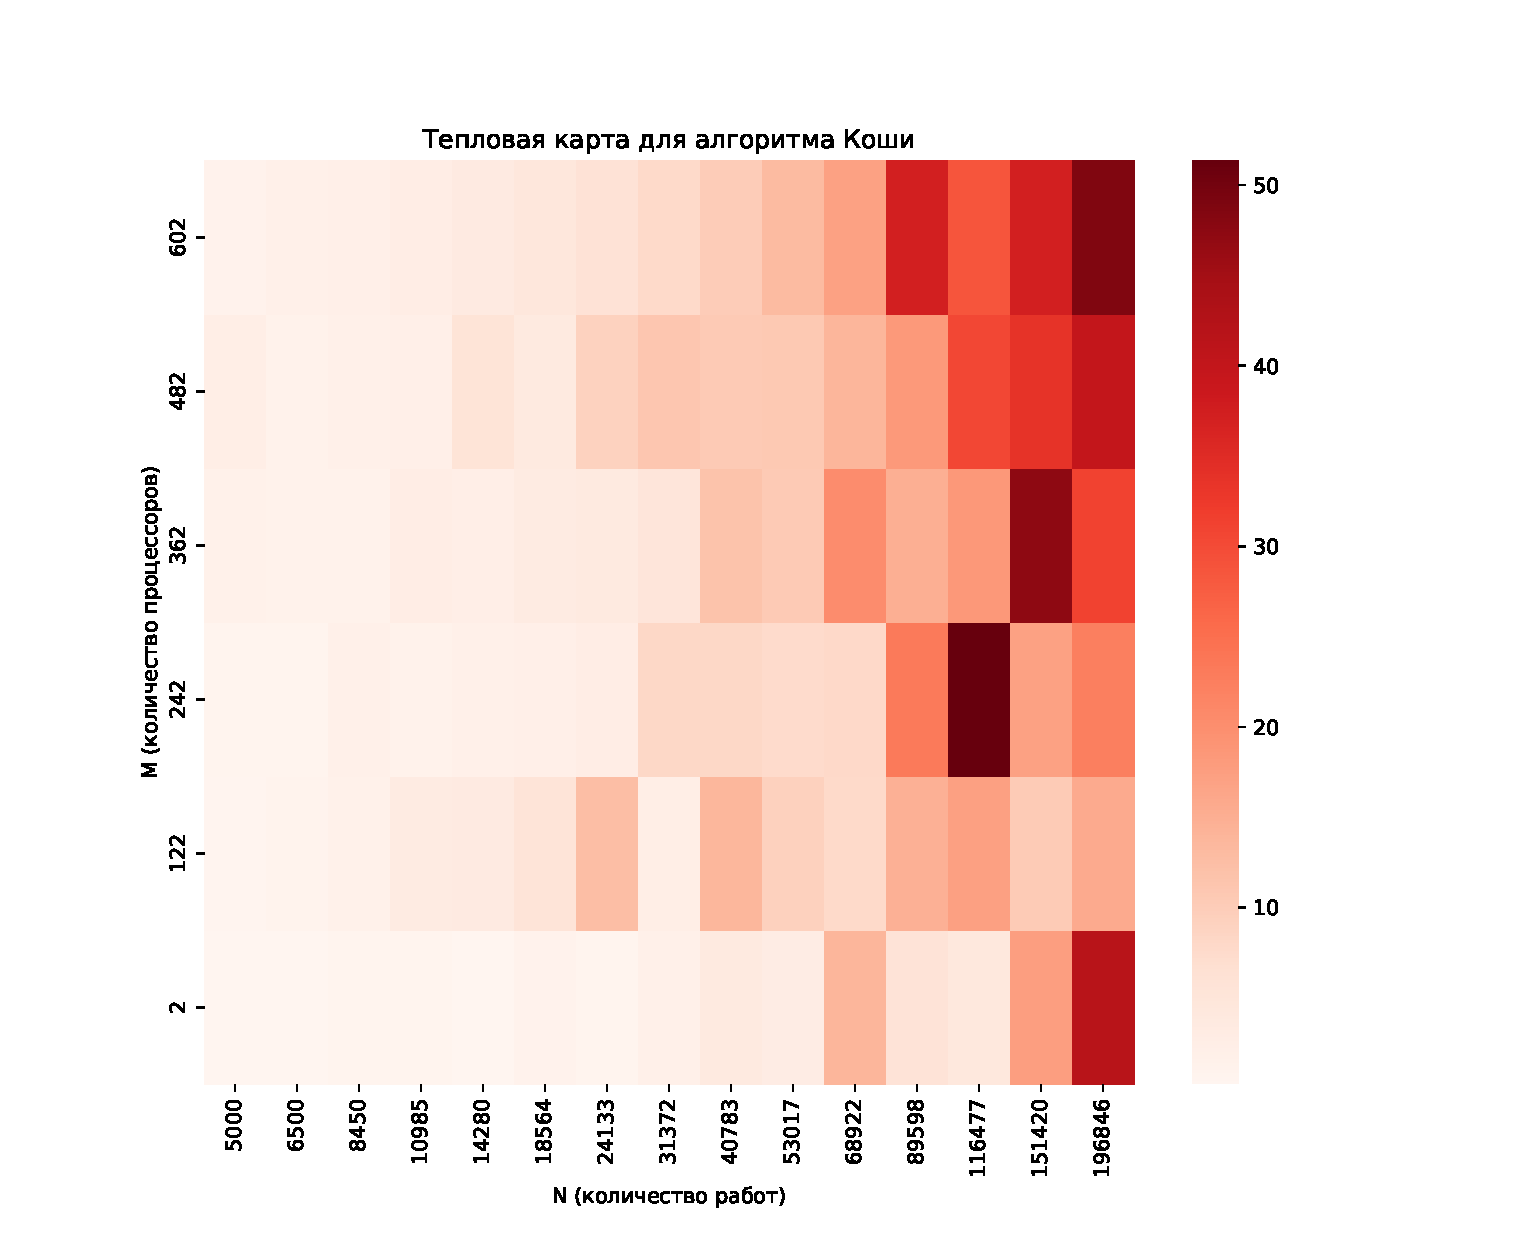
\includegraphics[width=\textwidth]{cauchy_heatmap.eps}
	    %\caption{}
	    \label{fig:cauchy}
	\end{figure}
	
	\begin{figure}[h]
	    \centering
	    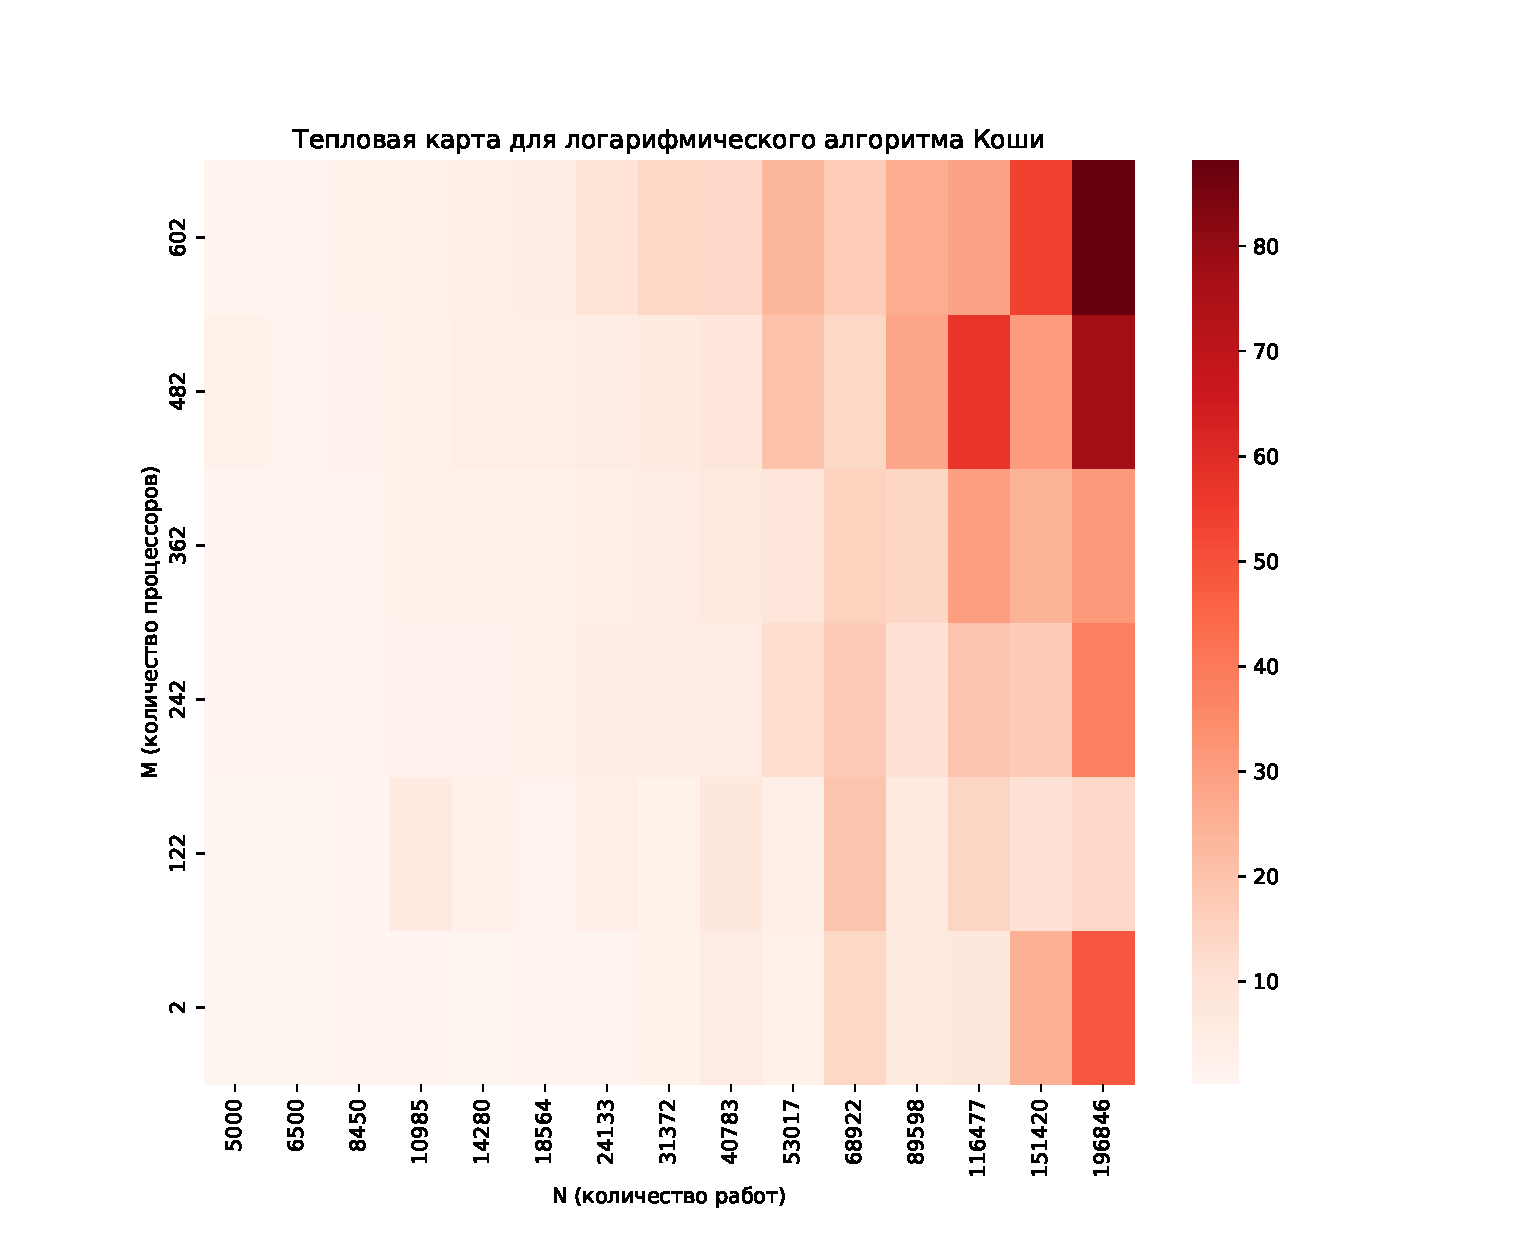
\includegraphics[width=\textwidth]{log_cauchy_heatmap.eps}
	    %\caption{}
	    \label{fig:log_cauchy}
	\end{figure}

	Исходя из полученных графиков можно сделать вывод, что время выполнения распределения
	растет при росте количества процессоров и количества задач.

	\section*{Исследование параллельного алгоритма}
\end{document}

